\documentclass{article}
\usepackage[utf8]{inputenc}
\usepackage[top=0.75in, bottom=0.75in, left=0.65in, right=0.65in]{geometry}
\usepackage{graphicx}
\usepackage{amsmath}
\usepackage{amsmath}
\usepackage{amssymb}
\usepackage{listings}
\usepackage[T1]{fontenc}
\usepackage[lighttt]{lmodern}
\usepackage{enumerate}

\usepackage{xcolor}
 
\definecolor{codegreen}{rgb}{0,0.6,0}
\definecolor{codegray}{rgb}{0.5,0.5,0.5}
\definecolor{codepurple}{rgb}{0.58,0,0.82}
\definecolor{backcolour}{rgb}{0.95,0.95,0.92}
 
\lstdefinestyle{mystyle}{
    backgroundcolor=\color{white},   
    commentstyle=\color{codegreen},
    keywordstyle=\color{magenta},
    numberstyle=\tiny\color{codegray},
    stringstyle=\color{codepurple},
    basicstyle=\ttfamily\footnotesize,
    breakatwhitespace=false,         
    breaklines=true,                 
    captionpos=b,                    
    keepspaces=true,                 
    numbers=left,                    
    numbersep=5pt,                  
    showspaces=false,                
    showstringspaces=false,
    showtabs=false,                  
    tabsize=2
}

\lstset{style=mystyle}
\usepackage{graphicx}
\graphicspath{{figure/}}


\newcommand*\lstinputpath[1]{\lstset{inputpath=#1}}
\lstinputpath{codes}
\title{Home Work 01: EAS 501}
\author{Sayem Khan}
\date{\today}


\begin{document}

\maketitle

\subsubsection*{Problem 1}
Consider $u(x, y)$ satisfying Laplace equation inside a rectangle $[0,1]\times[0,1]$ with the following Dirichlet boundary conditions $$u(0, y) = 3y-3,\hspace{5mm} u(1, y) = 4y-1, \hspace{5mm}   u(x,0) = 2x-3,\hspace{5mm}  u(x,1) = 3x$$ Solve this problem by the method of separation of variables and represent the solution explicitly.

\subsubsection*{Solution}
\begin{equation}
    u_{xx} + u_{yy} = 0
    \label{1eqn}
\end{equation}
Given Dirichlet boundary condition,
\begin{equation}
    \begin{split}
        u(0, x) &= 3y -3\\
        u(1, y) &= 4y -1\\
        u(x, 0) &= 2x - 3\\
        u(x, 1) &= 3x
    \end{split}
    \label{boundary}
\end{equation}
Assume,
$$
u(x,y) = d(x) + d(y)
$$
Then provide $\psi$ and $\phi$ are non-zero  functions. 
This implies,
\begin{equation*}
    \frac{\phi''(x)}{\phi(x)} = - \frac{\psi''(x)}{\psi(x)}
\end{equation*}
Then, $$
\phi(0) = 3y -3
$$
$$
\phi(1) = 4y -1
$$
For $$\lambda = 0$$

\begin{equation*}
    \begin{split}
        \phi(x) & = c_1 + c_2 x \\
        \phi(0) &= 3y -3 = c_1 \\
        \phi(1) &= 3y-3 + c_2 = 4y -1 \\
        c_2 &= y + 2
    \end{split}
\end{equation*}

% \subsubsection*{Problem 2} 
% Galilean Transformation. Consider the advection equation: $$
% \frac{\partial u}{\partial t} + c\frac{\partial u}{\partial x} = 0, \hspace{0.5cm} u_0(x) = u(0,x) = e^{-x^2}
% $$
% Consider a new $\hat{t}, \hat{x}$ coordinate system where,
% \begin{equation*}
%     \begin{split}
%       \hat{t}(t,x) &= t \\
%       \hat {x}(t,x) &= x - vt
%     \end{split}
% \end{equation*}
% and $v$ is a real number.

% \subsubsection*{Solution}
% \begin{enumerate}[(i)]
%     \item \begin{equation*}
%         \begin{split}
%             x' &= x - vt \\
%             \Rightarrow \frac{dx'}{dt} &= (c - v) \hspace{0.5cm} [\because \frac{dx}{dt} = c]
%         \end{split}
%     \end{equation*}
%     \begin{equation*}
%         \begin{split}
%             \frac{\partial u(t',x')}{\partial t'} &= \frac{\partial u}{\partial t'} + \frac{\partial u}{\partial x'}\frac{\partial x'}{\partial t'} \\
%             \frac{\partial u}{\partial t'} + (c -v) \frac{\partial u}{\partial x'} &= 0
%         \end{split}
%     \end{equation*}
    
%     \item \begin{equation*}
%         \begin{split}
%             c-v &= 0 \\
%             c &= v 
%         \end{split}
%     \end{equation*}
%     \item 
%     \begin{enumerate}
%         \item $v > c: $ Since, $c>0$, the characteristics curve has $(-)ve$ slope. Information is flowing form right to left. So, A boundary condition is needed in right.
%         \item $v = c:$ This is a stationary wave. No variation with time. So, boundary condition is required. 
%         \item $v < c: $ Since, $c>0$, Since, $c>0$, the characteristics curve has $(+)ve$ slope. Information is flowing form left to right. So, A boundary condition is needed in left.
%     \end{enumerate}
    
%     \item $$u(\hat{t}(t,x), \hat{x}(t,x) = e^{-(\hat{x}-(c-v)t )^{2}}$$
    
%     \item $$u(t,x) = e^{-(x -(c+v)t)^2} $$
    
% \end{enumerate}


% \subsubsection*{Problem 3}
% Method of characteristics, consider the advection equation,
% \begin{equation*}
%     \frac{\partial u}{\partial t} + 2\frac{\partial u}{\partial x} = 0
% \end{equation*}
% with the initial data $u(t = 0, x) = 5$ if $0 < x < 1$ otherwise $0$

% \subsubsection*{Solution}
% Using the method of characteristics, the characteristics curve,
% \begin{equation*}
% \begin{split}
%   \frac{d}{d t} x(t) &= 2 \\
%   x(t) &= 2t + K, \hspace{0.5cm} K = constant
% \end{split}
% \end{equation*}
% \begin{figure}[!]
%   \centering
%     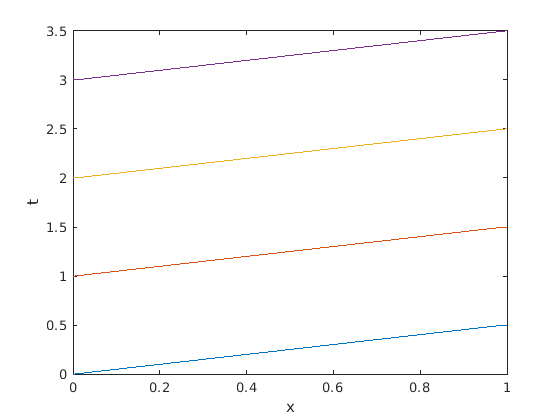
\includegraphics[width=0.85\textwidth]{t_x_plain.png}
%     \caption{Characteristics curve (Problem 3)} 
%     \label{EvsN}
% \end{figure}
% \vspace{1cm}
% Solution of the equation,
% \begin{equation*}
%     u(t,x) = \begin{cases}
% 5 & \text{ if } 2t < x < 1+2t \\ 
% 0 & \text{ if } otherwise 
% \end{cases}
% \end{equation*}
% For animation, please see the attached file.


% \subsubsection*{Problem 4}
% Advection equation,
% \begin{equation*}
%     \frac{\partial u}{\partial t} + 2\pi \frac{\partial u}{\partial x} = 0
% \end{equation*}
% With $u(0, x) = \sin(x)$, \hspace{0.5cm} $\sin(t, x = 0) =-sin(2\pi t)$ 

% \subsubsection*{Solution}
% Using method of characteristics,
% \begin{equation*}
%     u(t,x) = \begin{cases}
% sin(x - 2\pi t) & \text{ if } 2t < x < 2+2t \\ 
% 0 & \text{ if } otherwise 
% \end{cases}
% \end{equation*}
% \begin{figure}[!]
%   \centering
%     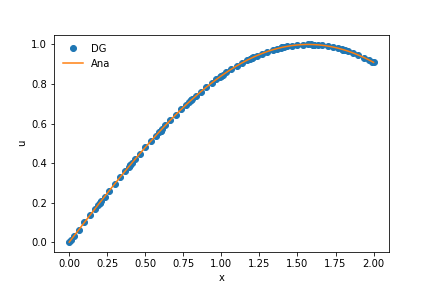
\includegraphics[width=0.85\textwidth]{DG_vs_ana.png}
%     \caption{Comparison between DG and analytical solution. (Problem 4)} 
%     \label{EvsN}
% \end{figure}


% % Specialize the general Monte Carlo integration method.
% % \subsubsection*{Solution}
% % The problem is,
% % \begin{equation}
% %   I_1 = \int_{-1}^{1}\frac{1}{1+x^2}dx
% %   \label{one}
% % \end{equation}
% % We need to write equation (\ref{one}) as 1-D Monte Carlo integration formula, that is,
% % \begin{equation}
% %   \hat{I}_{N} = V\frac{1}{N}\sum_{i = 1}^{N}\frac{1}{1+x_i^2} =2\frac{1}{N}\sum_{i = 1}^{N}\frac{1}{1+x_i^2}
% %   \label{two}
% % \end{equation}
% % where, $N\to \infty $, each $x_i$ is randomly and uniformly drawn from the interval $\left [ -1,1 \right ]$ and $V$ is the \textit{volume}, that is in this case,
% % \begin{equation*}
% %   V = \int_{-1}^{1}dx = x\mid^{1}_{-1} = 1-(-1) = 2
% % \end{equation*}
% % \subsubsection*{Problem b } 
% % The Pseudocode to compute the integration of equation \ref{two}. 
% % \subsubsection*{Solution}
% % \lstinputlisting[
% %   language   = python,
% %   basicstyle = \ttfamily,
% %   frame      = single,
% %   caption    = {Pseudocode for equation \ref{two}},
% % ]{mcAlgo.py}

% % \subsubsection*{Problem c } 
% % \subsubsection*{Solution}
% % The implementation of equation \ref{two} in C++ given below:
% % \lstinputlisting[
% %   language = C++,
% %   basicstyle = \ttfamily,
% %   frame      = single,
% %   caption    = {\textbf{monteCarlo.cpp}:  C++ implementation for equation (\ref{two}) with error calculation.},
% % ]{monteCarlo.cpp}
% % \vspace{13mm}
% % The bash script for Problem d, e, f given below:
% % \lstinputlisting[
% %   language = bash,
% %   basicstyle = \ttfamily,
% %   frame      = single,
% %   caption    = {Bash script \textbf{dataScript.sh} for execution and data generation in Problem d, e, f },
% % ]{dataScript.sh}

% % \subsubsection*{Problem d, e, f} 
% % \subsubsection*{Solution}
% % \begin{figure}[h!]
% %   \centering
% %     \includegraphics[width=0.85\textwidth]{Numerical_Intergration_Err_vs_Iteration.png}
% %     \caption{Numerical Integration Err vs Iteration: Problem d, e, f} 
% %     \label{EvsN}
% % \end{figure}
% % Here in the figure \ref{EvsN}, the Error vs Iteration is being plotted. The sequence of $N = 2^i$ for integers $i = 1, 2, 3,\cdots,30$ used as input. The theoretical error of the Monte Carlo integration is $E \propto N^{-1/2} $. \\
% % Here, the experiment run $200$ times and average error is being calculated.
% % \\
% % \\
% % \textbf{Problem e Solution:}
% % Here the error behaves like: 
% % $$
% % logE(N) = B + A\times log(N)
% % $$
% % If we assume $B = 0$ (since it is a constant), using the linear regression analysis, it is found that: 
% % $$A = -0.6049353724290725$$
% % But, it should be equal to $-0.5$. Since, several errors like rounding error and random number 
% % generation contributes error here. 
% % \subsubsection*{Problem g} 
% % \subsubsection*{Solution}
% % The execution time taken by \textbf{time.sh}.
% % \lstinputlisting[
% %   language = bash,
% %   basicstyle = \ttfamily,
% %   frame      = single,
% %   caption    = {\textbf{time.sh}: For execution and data generation in Problem g },
% % ]{time.sh}
% % \begin{figure}[h!]
% %   \centering
% %     \includegraphics[width=0.9\textwidth]{Time_vs_Number_of_Sample_point_curve}
% %     \caption{Time vs Iteration: Problem g} 
% %     \label{time}
% % \end{figure}

% % The run time is calculated by the Linux \textit{time} command. For first $18$ iteration, we got zero (0). Perhaps, CPU take some time in 'nano' second scale. So, \textit{time} command ignored that. The time data is plotted in \ref{time}. We have seen that the relation between iteration and time is linear. From the data, the best fitted model for time is: 
% % $$
% % T = 2.17309336\times 10^{-8} \times N + 5.4391834667749 \times 10^{-3} 
% % $$
% % where, T is time in second and N is number of iteration. Using this formula as well as using linear regression, it is found that time for $N = 2^{32}$ is $93.339$ seconds.
% % $$$$
\end{document}
